\documentclass{article}

\usepackage[top=1.5cm,bottom=0.5cm,left=0.5cm,right=0.5cm]{geometry}
\usepackage{xeCJK}
\usepackage{fontspec}
\usepackage{listings}
\usepackage{fancyhdr}
\usepackage{changepage}
\usepackage{color}
\usepackage{amsmath}
\usepackage{amssymb}
\usepackage{amsthm}
\usepackage{graphicx}
\usepackage{tikz}
\usepackage{algpseudocode}
\usepackage[shortlabels]{enumitem}
\usepackage{titlesec}
\usepackage{multicol}
\setCJKmainfont{Noto Serif CJK TC}
\setmonofont{Consolas}

\lstset{
language=C++,
basicstyle=\ttfamily\footnotesize,
tabsize=2,
breaklines=true,
breakatwhitespace=false,
escapeinside={\%*}{*)},
morekeywords={*}
}

\newcommand{\makegrid}{
\clearpage

\begin{center}
    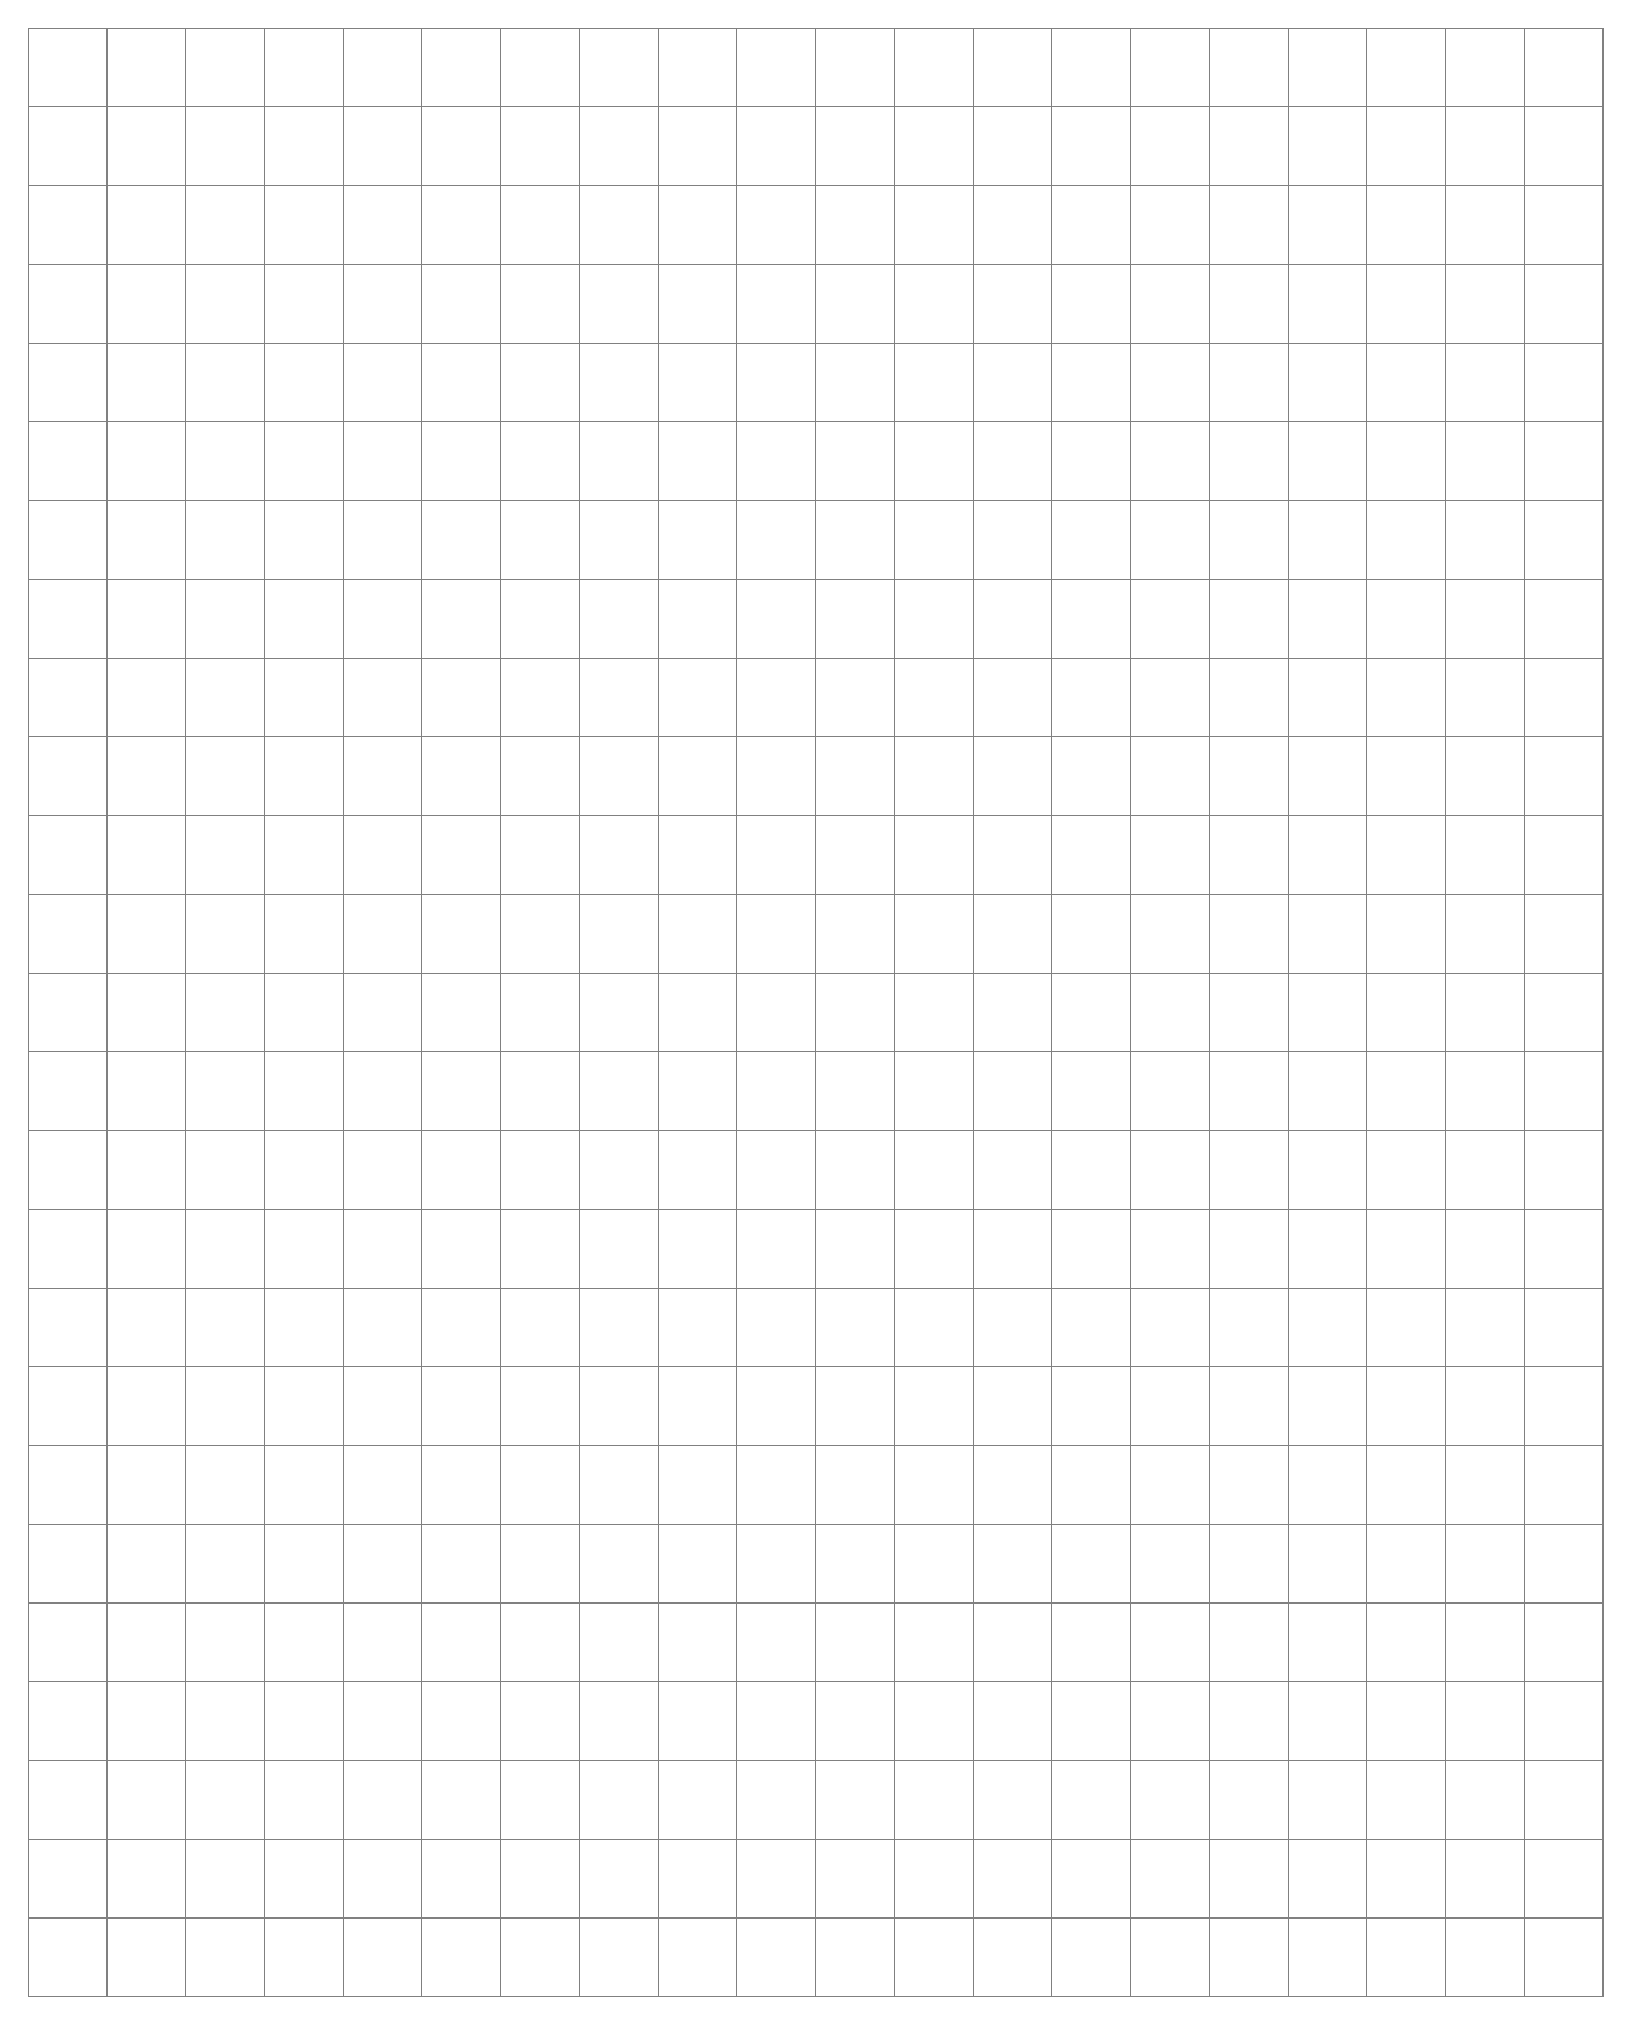
\begin{tikzpicture}
        \draw[step=1, gray, thin] (0,0) grid (20.0, 25.0);
    \end{tikzpicture}
\end{center}
}

\setlist[enumerate]{itemsep=0pt, parsep=0pt, topsep=0pt, leftmargin=10pt}
\setlist[itemize]{itemsep=0pt, parsep=0pt, topsep=0pt, leftmargin=10pt}

\titlespacing\section{0pt}{-2pt plus 0pt minus 2pt}{-1pt plus 0pt minus 2pt}
\titlespacing\subsection{0pt}{-2pt plus 0pt minus 2pt}{-1pt plus 0pt minus 2pt}
\titlespacing\subsubsection{0pt}{-2pt plus 0pt minus 2pt}{-1pt plus 0pt minus 2pt}

\begin{document}

\setlength\parindent{0pt}
\setlength\columnseprule{0.5pt}
\footnotesize


\pagestyle{fancy}
\fancyfoot{}
\fancyhead[L]{National Taiwan University}
\fancyhead[C]{\texttt{fruit\_advantages}}
\fancyhead[R]{\thepage}

\twocolumn

\setlength{\columnseprule}{0pt}
\begin{multicols}{2}
\tableofcontents
\end{multicols}
\setlength{\columnseprule}{0.5pt}

\section{Basic}

\subsection{Default Code}
\lstinputlisting{Basic/template.cpp}

\subsection{.vimrc}
\lstinputlisting{Basic/vimrc}

%\subsection{Windows Setup}
%\input{Basic/windows.tex}

%\subsection{Debug}
%\input{Basic/debug.tex}

\subsection{Fast IO}
\lstinputlisting{Basic/fastio.cpp}

\subsection{Random}
\lstinputlisting{Basic/random.cpp}

\subsection{Checker}
\lstinputlisting{Basic/checker.sh}

\subsection{PBDS Tree}
\lstinputlisting{Basic/pbds.cpp}

\subsection{Pragma}
\lstinputlisting{Basic/pragma.cpp}

\subsection{SVG Writer}
\lstinputlisting{Basic/SVG.cpp}

\section{Data Structure}

\subsection{Heavy-Light Decomposition}
\lstinputlisting{DataStructure/HLD.cpp}

%\subsection{Li-Chao Tree}
%\lstinputlisting{DataStructure/LiChao.cpp}

\subsection{Link Cut Tree}
\lstinputlisting{DataStructure/LinkCutTree.cpp}

\subsection{Treap}
\lstinputlisting{DataStructure/Treap.cpp}

\subsection{KD Tree}
\lstinputlisting{DataStructure/KDTree.cpp}

\subsection{Leftist Tree}
\lstinputlisting{DataStructure/LeftistTree.cpp}

\subsection{Convex 1D/1D}
\lstinputlisting{DataStructure/Convex1D1D.cpp}

%\subsection{Dynamic Convex Hull}
%\lstinputlisting{DataStructure/DynamicConvexHull.cpp}

\section{Flow \& Matching}

\subsection{Dinic}
\lstinputlisting{Flow_Matching/Dinic.cpp}

\subsection{Bounded Flow}
\lstinputlisting{Flow_Matching/BoundedFlow.cpp}

\subsection{MCMF}
\lstinputlisting{Flow_Matching/MCMF.cpp}

\subsection{Min Cost Circulation}
\lstinputlisting{Flow_Matching/MinCostCirculation.cpp}

\subsection{Gomory Hu}
\lstinputlisting{Flow_Matching/GomoryHu.cpp}

%\subsection{ISAP Algorithm}
%\lstinputlisting{Flow_Matching/isap.cpp}

\subsection{Stoer Wagner Algorithm}
\lstinputlisting{Flow_Matching/StoerWagner.cpp}

\subsection{Bipartite Matching}
\lstinputlisting{Flow_Matching/BipartiteMatching.cpp}

\subsection{Kuhn Munkres Algorithm}
\lstinputlisting{Flow_Matching/KuhnMunkres.cpp}

\subsection{Max Simple Graph Matching}
\lstinputlisting{Flow_Matching/MaxSimpleGraphMatching.cpp}

\subsection{Stable Marriage}
\input{Flow_Matching/StableMarriage.tex}

\subsection{Flow Model}
% \normalsize
\begin{itemize}
    %\itemsep-0.3em
    \item Maximum/Minimum flow with lower bound / Circulation problem
    %\vspace{-1em}
    \begin{enumerate}
        %\itemsep-0.3em
        \item Construct super source $S$ and sink $T$.
        \item For each edge $(x, y, l, u)$, connect $x \rightarrow y$ with capacity $u - l$.
        \item For each vertex $v$, denote by $in(v)$ the difference between the sum of incoming lower bounds and the sum of outgoing lower bounds.
        \item If $in(v) > 0$, connect $S \rightarrow v$ with capacity $in(v)$, otherwise, connect $v \rightarrow T$ with capacity $-in(v)$.
        \begin{itemize}
            %\itemsep-0.2em
            \item To maximize, connect $t \rightarrow s$ with capacity $\infty$ (skip this in circulation problem), and let $f$ be the maximum flow from $S$ to $T$. If $f \neq \sum_{v \in V, in(v) > 0}{in(v)}$, there's no solution. Otherwise, the maximum flow from $s$ to $t$ is the answer.
            \item To minimize, let $f$ be the maximum flow from $S$ to $T$. Connect $t \rightarrow s$ with capacity $\infty$ and let the flow from $S$ to $T$ be $f^\prime$. If $f + f^\prime \neq \sum_{v \in V, in(v) > 0}{in(v)}$, there's no solution. Otherwise, $f^\prime$ is the answer.
        \end{itemize}
        \item The solution of each edge $e$ is $l_e + f_e$, where $f_e$ corresponds to the flow of edge $e$ on the graph.
    \end{enumerate}
    \item Construct minimum vertex cover from maximum matching $M$ on bipartite graph $(X, Y)$
    %\vspace{-1em}
    \begin{enumerate}
        %\itemsep-0.3em
        \item Redirect every edge: $y \rightarrow x$ if $(x, y) \in M$, $x \rightarrow y$ otherwise.
        \item DFS from unmatched vertices in $X$.
        \item $x \in X$ is chosen iff $x$ is unvisited.
        \item $y \in Y$ is chosen iff $y$ is visited.
    \end{enumerate}
    \item Minimum cost cyclic flow
    %\vspace{-0.5em}
    \begin{enumerate}
        %\itemsep-0.3em
        \item Consruct super source $S$ and sink $T$
        \item For each edge $(x, y, c)$, connect $x \rightarrow y$ with $(cost, cap) = (c, 1)$ if $c > 0$, otherwise connect $y \rightarrow x$ with $(cost, cap) = (-c, 1)$
        \item For each edge with $c < 0$, sum these cost as $K$, then increase $d(y)$ by 1, decrease $d(x)$ by 1
        \item For each vertex $v$ with $d(v) > 0$, connect $S \rightarrow v$ with $(cost, cap) = (0, d(v))$
        \item For each vertex $v$ with $d(v) < 0$, connect $v \rightarrow T$ with $(cost, cap) = (0, -d(v))$
        \item Flow from $S$ to $T$, the answer is the cost of the flow $C + K$
    \end{enumerate}
    \item Maximum density induced subgraph
    %\vspace{-1em}
    \begin{enumerate}
        %\itemsep-0.3em
        \item Binary search on answer, suppose we're checking answer $T$
        \item Construct a max flow model, let $K$ be the sum of all weights
        \item Connect source $s \rightarrow v$, $v \in G$ with capacity $K$
        \item For each edge $(u, v, w)$ in $G$, connect $u \rightarrow v$ and $v \rightarrow u$ with capacity $w$
        \item For $v \in G$, connect it with sink $v \rightarrow t$ with capacity $K + 2T - (\sum_{e \in E(v)}{w(e)}) - 2w(v)$
        \item $T$ is a valid answer if the maximum flow $f < K \lvert V \rvert$
    \end{enumerate}
    \item Minimum weight edge cover
    %\vspace{-1em}
    \begin{enumerate}
        %\itemsep-0.3em
      \item For each $v \in V$ create a copy $v^\prime$, and connect $u^\prime \to v^\prime$ with weight $w(u, v)$.
      \item Connect $v \to v^\prime$ with weight $2\mu(v)$, where $\mu(v)$ is the cost of the cheapest edge incident to $v$.
      \item Find the minimum weight perfect matching on $G^\prime$.
    \end{enumerate}
    \item Project selection problem
    %\vspace{-1em}
    \begin{enumerate}
      %\itemsep-0.3em
      \item If $p_v > 0$, create edge $(s, v)$ with capacity $p_v$; otherwise, create edge $(v, t)$ with capacity $-p_v$.
      \item Create edge $(u, v)$ with capacity $w$ with $w$ being the cost of choosing $u$ without choosing $v$.
      \item The mincut is equivalent to the maximum profit of a subset of projects.
    \end{enumerate}
    \item Dual of minimum cost maximum flow
    %\vspace{-1em}
    \begin{enumerate}
      %\itemsep-0.3em
      \item Capacity $c_{uv}$, Flow $f_{uv}$, Cost $w_{uv}$, Required Flow difference for vertex $b_u$.
      \item If all $w_{uv}$ are integers, then optimal solution can happen when all $p_u$ are integers.
    \end{enumerate}
    $$
    \begin{aligned}\min\sum_{uv} w_{uv}f_{uv} \\ -f_{uv} \geq -c_{uv} \\ \sum_{v} f_{vu} - \sum_{v} f_{uv} = -b_u\end{aligned}
    \Leftrightarrow
    \begin{aligned}\min\sum_{u} b_up_u + \sum_{uv}c_{uv}\max(0, p_v - p_u - w_{uv}) \\ p_u \geq 0 \end{aligned}
    $$
    %\item 0/1 quadratic programming
    %%\vspace{-1em}
    %\[ \sum_x{c_xx} + \sum_y{c_y\bar{y}} + \sum_{xy}c_{xy}x\bar{y} + \sum_{xyx^\prime y^\prime}c_{xyx^\prime y^\prime}(x\bar{y} + x^\prime\bar{y^\prime}) \]
    %can be minimized by the mincut of the following graph:
    %\begin{enumerate}
    %  %\itemsep-0.3em
    %  \item Create edge $(x, t)$ with capacity $c_x$ and create edge $(s, y)$ with capacity $c_y$.
    %  \item Create edge $(x, y)$ with capacity $c_{xy}$.
    %  \item Create edge $(x, y)$ and edge $(x^\prime, y^\prime)$ with capacity $c_{xyx^\prime y^\prime}$.
    %\end{enumerate}
\end{itemize}


\section{Geometry}

\subsection{Geometry Template}
\lstinputlisting{Geometry/GeometryTemplate.cpp}

%\subsection{Convex Hull}
%\lstinputlisting{Geometry/ConvexHull.cpp}

\subsection{Polar Angle Comparator}
\lstinputlisting{Geometry/PolarAngleComp.cpp}

\subsection{Minkowski Sum}
\lstinputlisting{Geometry/MinkowskiSum.cpp}

\subsection{Intersection of Circle and Convex Polygon}
\lstinputlisting{Geometry/CircleConvexIntersection.cpp}

\subsection{Intersection of Circles}
\lstinputlisting{Geometry/CircleCircleIntersection.cpp}

\subsection{Tangent Line of Circles}
\lstinputlisting{Geometry/CircleCircleTangent.cpp}

\subsection{Intersection of Line and Convex Polygon}
\lstinputlisting{Geometry/ConvexLineIntersection.cpp}

\subsection{Intersection of Line and Circle}
\lstinputlisting{Geometry/CircleLineIntersection.cpp}

\subsection{Point in Circle}
\lstinputlisting{Geometry/PointInCircle.cpp}

\subsection{Point in Convex}
\lstinputlisting{Geometry/PointInConvex.cpp}

\subsection{Half Plane Intersection}
\lstinputlisting{Geometry/HalfPlaneIntersection.cpp}

\subsection{Minimum Enclosing Circle}
\lstinputlisting{Geometry/MinimumEnclosingCircle.cpp}

\subsection{3D Point}
\lstinputlisting{Geometry/3DPoint.cpp}

\subsection{ConvexHull3D}
\lstinputlisting{Geometry/ConvexHull3D.cpp}

\subsection{Delaunay Triangulation}
\lstinputlisting{Geometry/DelaunayTriangulation.cpp}

\subsection{Voronoi Diagram}
\lstinputlisting{Geometry/VoronoiDiagram.cpp}

\subsection{Polygon Union}
\lstinputlisting{Geometry/PolyUnion.cpp}

\subsection{Tangent Point to Convex Hull}
\lstinputlisting{Geometry/TangentPointToHull.cpp}

\subsection{Heart}
\lstinputlisting{Geometry/Heart.cpp}

\subsection{Rotating Sweep Line}
\lstinputlisting{Geometry/RotatingSweepLine.cpp}

%\subsection{ConvexHullDP}
%\lstinputlisting{Geometry/ConvexHullDP.cpp}

\subsection{Vector In Poly}
\lstinputlisting{Geometry/VectorInPoly.cpp}

\section{Graph}

\subsection{BCC}
\lstinputlisting{Graph/BCC.cpp}

\subsection{SCC}
\lstinputlisting{Graph/SCC.cpp}

\subsection{2-SAT}
\lstinputlisting{Graph/2SAT.cpp}

\subsection{Dominator Tree}
\lstinputlisting{Graph/DominatorTree.cpp}

\subsection{Virtual Tree}
\lstinputlisting{Graph/VirtualTree.cpp}

%\subsection{Directed Minimum Spanning Tree}
%\lstinputlisting{Graph/DirectedMST.cpp}

\subsection{Fast DMST}
\lstinputlisting{Graph/FastDMST.cpp}

\subsection{Vizing}
\lstinputlisting{Graph/Vizing.cpp}

\subsection{Maximum Clique}
\lstinputlisting{Graph/MaximumClique.cpp}

\subsection{Number of Maximal Clique}
\lstinputlisting{Graph/NumberOfMaximalClique.cpp}

\subsection{Minimum Mean Cycle}
\lstinputlisting{Graph/MinimumMeanCycle.cpp}

\subsection{Minimum Steiner Tree}
\lstinputlisting{Graph/MinimumSteinerTree.cpp}

\section{Math}

\subsection{Extended Euclidean Algorithm}
\lstinputlisting{Math/ExtGCD.cpp}

\subsection{Floor \& Ceil}
\lstinputlisting{Math/floor_ceil.cpp}

\subsection{Legendre}
\lstinputlisting{Math/Legendre.cpp}

\subsection{Simplex}
\lstinputlisting{Math/Simplex.cpp}

\subsection{Floor Sum}
\lstinputlisting{Math/FloorSum.cpp}

\subsection{DiscreteLog}
\lstinputlisting{Math/DiscreteLog.cpp}

\subsection{Miller Rabin \& Pollard Rho}
\lstinputlisting{Math/MillerRabin_PollardRho.cpp}

\subsection{XOR Basis}
\lstinputlisting{Math/Basis.cpp}

\subsection{Linear Equation}
\lstinputlisting{Math/LinearEquation.cpp}

\subsection{Chinese Remainder Theorem}
\lstinputlisting{Math/ChineseRemainderTheorem.cpp}

\subsection{Sqrt Decomposition}
\lstinputlisting{Math/SqrtDecomposition.cpp}

\section{Misc}

%\subsection{Fraction}
%\lstinputlisting{Misc/Fraction.cpp}

\subsection{Cyclic Ternary Search}
\lstinputlisting{Misc/cyc_tsearch.cpp}

\subsection{Matroid}
% From IOIC 2021,2022
%我們稱一個二元組 $M = (E, \mathcal{I})$ 為一個擬陣,
%其中 $\mathcal{I} \subseteq 2^E$ 為 $E$ 的子集所形成的\textbf{非空}集合,若:
%
%\begin{itemize}
%    \item 若 $S \in \mathcal{I}$ 以及 $S^\prime \subsetneq S$,則
%        $S^\prime \in \mathcal{I}$
%    \item 對於 $S_1, S_2 \in \mathcal{I}$ 滿足 $|S_1| < |S_2|$,存在
%        $e \in S_2 \setminus S_1$ 使得 $S_1 \cup \{e\} \in \mathcal{I}$
%\end{itemize}
%
%除此之外,我們有以下的定義:
%
%\begin{itemize}
%    \item 位於 $\mathcal{I}$ 中的集合我們稱之為獨立集(independent set),反之不在
%        $\mathcal{I}$ 中的我們稱為相依集(dependent set)
%    \item 極大的獨立集為基底(base)、極小的相依集為迴路(circuit)
%    \item 一個集合 $Y$ 的秩(rank)$r(Y)$ 為該集合中最大的獨立子集,也就是
%        $r(Y) = \max\{|X| \mid X \subseteq Y \text{ 且 } X \in \mathcal{I} \}$
%\end{itemize}
%
%性質:
%\begin{enumerate}
%    \item $X \subseteq Y \land Y \in \mathcal I \implies X \in \mathcal I$
%    \item $X \subseteq Y \land X \notin \mathcal I \implies Y \notin \mathcal I$
%    \item 若 $B$ 與 $B'$ 皆是基底且 $B \subseteq B'$,則 $B=B'$\\
%          若 $C$ 與 $C'$ 皆是迴路且 $C \subseteq C'$,則 $C=C'$
%    \item $e \in E \land X \subseteq E \implies r(X) \leq r(X \cup \{e\}) \leq r(X) + 1$ i.e. 加入一個元素後秩不會降底,最多增加 1
%    \item $\forall Y \subseteq E, \exists X \subseteq Y, r(X)=\lvert X \rvert = r(Y)$
%\end{enumerate}
%
%一些等價的性質:
%\begin{enumerate}
%    \item 對於所有 $X \subseteq E$,$X$ 的極大獨立子集都有相同的大小
%    \item 對於 $B_1,B_2 \in \mathcal B \land B_1 \neq B_2$,
%        對於所有 $e_1 \in B_1 \setminus B_2$,
%        存在 $e_2 \in B_2 \setminus B_1$ 使得 $(B_1 \setminus \{e_1\}) \cup \{e_2\} \in \mathcal B$
%    \item 對於 $X,Y \in \mathcal I$ 且 $\lvert X \rvert < \lvert Y \rvert$,存在 $e \in Y \setminus X$ 使得 $X \cup \{e\} \in \mathcal B$
%    \item 如果 $r(X \cup \{e_1\}) = r(X \cup \{e_2\}) = r(X)$,則 $r(X \cup \{e_1,e_2\}) = r(X)$。
%        如果 $r(X \cup \{e\}) = r(X)$ 對於所有 $e \in E'$ 都成立,則 $r(X \cup E') = r(X)$。
%\end{enumerate}

$M=(E,\mathcal{I})$, where $\mathcal{I} \subseteq 2^E$ is nonempty, is a matroid if:
\begin{itemize}
    \item If $S \in \mathcal{I}$ and $S^\prime \subsetneq S$, then $S^\prime \in \mathcal{I}$.
    \item For $S_1,S_2 \in \mathcal{I}$ s.t. $\lvert S_1 \rvert < \lvert S_2 \rvert$,
        there exists $e \in S_2 \setminus S_1$ s.t. $S_1 \cup \{e\} \in \mathcal{I}$.
\end{itemize}

Matroid intersection:

Start from $S = \emptyset$. In each iteration, let 
%\vspace{-0.5em}
\begin{itemize}
    %\itemsep-0.5em
    \item $Y_1 = \{x \not\in S \mid S \cup \{x\} \in \mathcal{I}_1 \}$
    \item $Y_2 = \{x \not\in S \mid S \cup \{x\} \in \mathcal{I}_2 \}$
\end{itemize}
If there exists $x \in Y_1 \cap Y_2$, insert $x$ into $S$. Otherwise for each $x \in S, y \not\in S$, create edges
%\vspace{-0.5em}
\begin{itemize}
    %\itemsep-0.5em
    \item $x \to y$ if $S - \{x\} \cup \{y\} \in \mathcal{I}_1$.
    \item $y \to x$ if $S - \{x\} \cup \{y\} \in \mathcal{I}_2$.
\end{itemize}
Find a \textit{shortest} path (with BFS) starting from a vertex in $Y_1$ and ending at a vertex in $Y_2$ which doesn't pass through any other vertices in $Y_2$, and alternate the path. The size of $S$ will be incremented by 1 in each iteration. For the weighted case, assign weight $w(x)$ to vertex $x$ if $x \in S$ and $-w(x)$ if $x \not\in S$. Find the path with the minimum number of edges among all minimum length paths and alternate it.



\section{Polynomial}

\subsection{FWHT}
\lstinputlisting{Polynomial/FWHT.cpp}

\subsection{FFT}
\lstinputlisting{Polynomial/FFT.cpp}

\subsection{NTT}
\lstinputlisting{Polynomial/NTT.cpp}

\subsection{Polynomial Operation}
\lstinputlisting{Polynomial/PolynomialOperation.cpp}

\subsection{Generating Function}
% From IOIC 2021
\subsubsection{Ordinary Generating Function}

\begin{itemize}
    \item $C(x) = A(rx)$: $c_n = r^na_n$ 的一般生成函數。
    \item $C(x) = A(x) + B(x)$: $c_n = a_n + b_n$ 的一般生成函數。
    \item $C(x) = A(x)B(x)$: $c_n = \sum\limits_{i = 0}^n a_ib_{n - i}$ 的一般生成函數。
    \item $C(x) = A(x)^k$: $c_n = \sum\limits_{i_1 + i_2 + \ldots + i_k = n} a_{i_1}a_{i_2} \ldots a_{i_k}$ 的一般生成函數。
    \item $C(x) = xA(x)'$: $c_n = na_n$ 的一般生成函數。
    \item $C(x) = \frac{A(x)}{1 - x}$: $c_n = \sum\limits_{i = 0}^n a_i$ 的一般生成函數。
	\item $C(x) = A(1) + x\frac{A(1) - A(x)}{1-x}$: $c_n = \sum\limits_{i=n}^{\infty} a_i$ 的一般生成函數。
\end{itemize}

常用展開式
\begin{itemize}
    \item $\frac{1}{1 - x} = 1 + x + x^2 + \ldots + x^n + \ldots$
    \item $(1 + x)^a = \sum\limits_{n = 0}^{\infty} \binom{a}{n} x^n, \, \binom{a}{n} = \frac{a(a - 1)(a - 2) \ldots (a - n + 1)}{n!}$.
\end{itemize}

常見生函
\begin{itemize}
	\item 卡特蘭數:$f(x) = \frac{1 - \sqrt{1-4x}}{2x}$
\end{itemize}

\subsubsection{Exponential Generating Function}

$a_0,a_1,\dots$ 的指數生成函數:

\[\hat A(x) = \sum_{i=0}^\infty \frac{a_i}{i!} = a_0 + a_1x + \frac{a_2}{2!}x^2 + \frac{a_3}{3!}x^3 + \dots\]

\begin{itemize}
    \item $\hat C(x) = \hat A(x) + \hat B(x)$: $c_n=a_n+b_n$ 的指數生成函數
    \item $\hat C(x) = \hat A^{(k)}(x)$: $c_n=a_{n+k}$ 的指數生成函數
    \item $\hat C(x) = x\hat A(x)$: $c_n=na_n$ 的指數生成函數
    \item $\hat C(x) = \hat A(x)\hat B(x)$: $c_n=\sum_{k=0}^n \binom{n}{i} a_kb_{n-k}$ 的指數生成函數
    \item $\hat C(x) = \hat A(x)^k$: $\sum\limits_{i_1+i_2+\dots+i_k=n} \binom{n}{i_1,i_2,\dots,i_k}a_ia_{i_2}\dots a_{i_k}$ 的指數生成函數
	\item $\hat C(x) = \exp(A(x))$: 假設 $A(x)$ 是一個分量 (component) 的生成函數,那 $\hat C(x)$ 是將 $n$ 個有編號的東西分成若干個分量的指數生成函數
\end{itemize}

Lagrange's Inversion Formula

如果 F 跟 G 互反,H 為任意 FPS,則

\[ n [x^n] G(x) = [x^{-1}]\frac{1}{F(x)^{n}}\]
\[ n [x^n] H(G(x)) = [x^{-1}] H'(x) \frac{1}{F(x)^{n}}\]


\subsection{Bostan Mori}
\lstinputlisting{Polynomial/BostanMori.cpp}

\section{String}

\subsection{KMP Algorithm}
\lstinputlisting{String/KMP.cpp}

\subsection{Manacher Algorithm}
\lstinputlisting{String/Manacher.cpp}

\subsection{Lyndon Factorization}
\lstinputlisting{String/Duval.cpp}

\subsection{Suffix Array}
\lstinputlisting{String/SA.cpp}

\subsection{Suffix Automaton}
\lstinputlisting{String/SAM.cpp}

\subsection{Z-value Algorithm}
\lstinputlisting{String/Zvalue.cpp}

\subsection{Main Lorentz}
\lstinputlisting{String/MainLorentz.cpp}

\subsection{AC Automaton}
\lstinputlisting{String/Aho_Corasick.cpp}

\subsection{Palindrome Automaton}
\lstinputlisting{String/PAM.cpp}

\section{Formula}
% modified from kactl
\subsection{Recurrences}
If $a_n = c_1 a_{n-1} + \dots + c_k a_{n-k}$, and $r_1, \dots, r_k$ are distinct roots of $x^k + c_1 x^{k-1} + \dots + c_k$, there are $d_1, \dots, d_k$ s.t.
\[a_n = d_1r_1^n + \dots + d_kr_k^n. \]
Non-distinct roots $r$ become polynomial factors, e.g. $a_n = (d_1n + d_2)r^n$.

\subsection{Geometry}

\subsubsection{Rotation Matrix}

\[ \begin{pmatrix}
    \cos \theta & -\sin \theta \\
    \sin \theta & \cos \theta
\end{pmatrix} \]

\begin{itemize}
    \item rotate $90^\circ$: $(x,y) \to (-y, x)$
    \item rotate $-90^\circ$: $(x,y) \to (y, -x)$
\end{itemize}

\subsubsection{Triangles}
Side lengths: $a,b,c$\\
Semiperimeter: $p=\dfrac{a+b+c}{2}$\\
Area: $A=\sqrt{p(p-a)(p-b)(p-c)}$\\
Circumradius: $R=\dfrac{abc}{4A}$\\
Inradius: $r=\dfrac{A}{p}$\\
Length of median (divides triangle into two equal-area triangles): $m_a=\tfrac{1}{2}\sqrt{2b^2+2c^2-a^2}$\\
Length of bisector (divides angles in two): $s_a=\sqrt{bc\left(1-\left(\dfrac{a}{b+c}\right)^2\right)}$\\
Law of sines: $\dfrac{\sin\alpha}{a}=\dfrac{\sin\beta}{b}=\dfrac{\sin\gamma}{c}=\dfrac{1}{2R}$\\
Law of cosines: $a^2=b^2+c^2-2bc\cos\alpha$\\
Law of tangents: $\dfrac{a+b}{a-b}=\dfrac{\tan\dfrac{\alpha+\beta}{2}}{\tan\dfrac{\alpha-\beta}{2}}$\\
%Incenter:\\
%$P_1=(x_1,y_1),P_2=(x_2,y_2),P_3=(x_3,y_3)$\\
%$s_1=\overline{P_2P_3}, s_2=\overline{P_1P_3}, s_3=\overline{P_1P_2}$ \\
%$\dfrac{s_1P_1 + s_2P_2 + s_3P_3}{s_1+s_2+s_3}$\\
%Circumcenter:\\
%$P_0=(0,0),P_1=(x_1,y_1),P_2=(x_2,y_2)$\\
%$x_c=\frac{1}{2} \times \dfrac{y_2(x_1^2+y_1^2)-y_1(x_2^2+y_2^2)}{-x_2y_1+x_1y_2}$\\
%$y_c=\frac{1}{2} \times \dfrac{x_2(x_1^2+y_1^2)-x_1(x_2^2+y_2^2)}{-x_1y_2+x_2y_1}$\\
%Check if $(x_0,y_0)$ is in the circumcircle:\\
%\[\begin{vmatrix}
%x_1-x_0 & y_1-y_0 & (x_1^2+y_1^2)-(x_0^2+y_0^2) \\
%x_2-x_0 & y_2-y_0 & (x_2^2+y_2^2)-(x_0^2+y_0^2) \\
%x_3-x_0 & y_3-y_0 & (x_3^2+y_3^2)-(x_0^2+y_0^2) \\
%\end{vmatrix}\]
%$0$: on edge, $>0$: inside, $<0$: outside\\

\subsubsection{Quadrilaterals}
With side lengths $a,b,c,d$, diagonals $e, f$, diagonals angle $\theta$, area $A$ and
magic flux $F=b^2+d^2-a^2-c^2$:

\[ 4A = 2ef \cdot \sin\theta = F\tan\theta = \sqrt{4e^2f^2-F^2} \]

 For cyclic quadrilaterals the sum of opposite angles is $180^\circ$,
$ef = ac + bd$, and $A = \sqrt{(p-a)(p-b)(p-c)(p-d)}$.

\subsubsection{Spherical coordinates}
\begin{center}
\includegraphics[width=25mm]{sphericalCoordinates.pdf}
\end{center}
\[\begin{array}{cc}
x = r\sin\theta\cos\phi & r = \sqrt{x^2+y^2+z^2}\\
y = r\sin\theta\sin\phi & \theta = \textrm{acos}(z/\sqrt{x^2+y^2+z^2})\\
z = r\cos\theta & \phi = \textrm{atan2}(y,x)
\end{array}\]

\subsubsection{Green's Theorem}

\[ \iint_D \left( \frac{\partial Q}{\partial x} - \frac{\partial P}{\partial y} \right) dxdy
= \oint_{L^+} (Pdx + Qdy)\]

\[ \text{Area} = \frac{1}{2} \oint_L x\ dy - y\ dx \]

Circular sector:

\begin{align*}
    x &= x_0 + r\cos\theta \\
    y &= y_0 + r\sin\theta \\
    A &= r \int_\alpha^\beta (x_0 + \cos\theta)\cos\theta + (y_0 + \sin\theta)\sin\theta\ d\theta \\
      &= r (r \theta + x_0 \sin\theta - y_0 \cos\theta) \rvert_\alpha^\beta
\end{align*}

\subsubsection{Point-Line Duality}

\[ p=(a,b) \leftrightarrow p^*: y=ax-b \]

\begin{itemize}
    \item $p \in l \iff l^* \in p^*$
    \item $p_1, p_2, p_3$ are collinear $\iff$ $p_1^*, p_2^*, p_3^*$ intersect at a point
    \item $p$ lies above $l$ $\iff$ $l^*$ lies above $p^*$
    \item lower convex hull $\leftrightarrow$ upper envelope
\end{itemize}

\subsection{Trigonometry}
\begin{align*}
    \sinh x = \frac{1}{2}(e^x - e^{-x}) &&& \cosh x = \frac{1}{2}(e^x + e^{-x}) \\
    \sin n\pi = 0 &&& \cos n\pi = (-1)^n
\end{align*}
\begin{align*}
\sin(\alpha+\beta)&{}=\sin \alpha\cos \beta+\cos \alpha\sin \beta\\
\cos(\alpha+\beta)&{}=\cos \alpha\cos \beta-\sin \alpha\sin \beta\\
\sin(2\alpha) &{}=2\cos \alpha \sin \alpha \\
\cos(2\alpha) &{}=\cos^2 \alpha - \sin^2 \alpha \\
         &{}=2\cos^2 \alpha - 1 \\
         &{}=1 - 2 \sin^2 \alpha
\end{align*}
\begin{align*}
\tan(\alpha+\beta)&{}=\dfrac{\tan \alpha+\tan \beta}{1-\tan \alpha\tan \beta}\\
\sin \alpha+\sin \beta&{}=2\sin\dfrac{\alpha+\beta}{2}\cos\dfrac{\alpha-\beta}{2}\\
\cos \alpha+\cos \beta&{}=2\cos\dfrac{\alpha+\beta}{2}\cos\dfrac{\alpha-\beta}{2} \\
\sin \alpha \sin \beta&{}=\frac{1}{2}(\cos(\alpha - \beta) - \cos(\alpha + \beta)) \\
\sin \alpha \cos \beta&{}=\frac{1}{2}(\sin(\alpha + \beta) + \sin(\alpha - \beta)) \\
\cos \alpha \sin \beta&{}=\frac{1}{2}(\sin(\alpha + \beta) - \sin(\alpha - \beta)) \\
\cos \alpha \cos \beta&{}=\frac{1}{2}(\cos(\alpha - \beta) + \cos(\alpha + \beta))
\end{align*}
\[ (V+W)\tan(\alpha-\beta)/2{}=(V-W)\tan(\alpha+\beta)/2 \]
where $V, W$ are lengths of sides opposite angles $\alpha, \beta$.
\begin{align*}
	a\cos x+b\sin x&=r\cos(x-\phi)\\
	a\sin x+b\cos x&=r\sin(x+\phi)
\end{align*}
where $r=\sqrt{a^2+b^2}, \phi=\operatorname{atan2}(b,a)$.

\subsection{Derivatives/Integrals}

Integration by parts:
\[\int_a^bf(x)g(x)dx = [F(x)g(x)]_a^b-\int_a^bF(x)g'(x)dx\]

\begin{align*}
	\dfrac{d}{dx}\arcsin x = \dfrac{1}{\sqrt{1-x^2}} &&& \dfrac{d}{dx}\arccos x = -\dfrac{1}{\sqrt{1-x^2}} \\
	\dfrac{d}{dx}\tan x = 1+\tan^2 x &&& \dfrac{d}{dx}\arctan x = \dfrac{1}{1+x^2} \\
	\int\tan ax = -\dfrac{\ln|\cos ax|}{a} &&& \int x\sin ax = \dfrac{\sin ax-ax \cos ax}{a^2} \\
	\int e^{-x^2} = \frac{\sqrt \pi}{2} \text{erf}(x) &&& \int xe^{ax} = \frac{e^{ax}}{a^2}(ax-1) \\
    \int \sin^2(x) = \frac{x}{2} - \frac{1}{4} \sin 2x &&& \int \sin^3 x = \frac{1}{12}\cos 3x - \frac{3}{4} \cos x \\
    \int \cos^2(x) = \frac{x}{2} + \frac{1}{4} \sin 2x &&& \int \cos^3 x = \frac{1}{12}\sin 3x + \frac{3}{4} \sin x \\
    \int x \sin x = \sin x - x \cos x &&& \int x \cos x = \cos x + x \sin x \\
    \int xe^x = e^x(x - 1) &&& \int x^2 e^x = e^x(x^2 - 2x + 2) \\
\end{align*}
\begin{align*}
    \int x^2 \sin x &= 2x \sin x - (x^2 - 2) \cos x \\
    \int x^2 \cos x &= 2x \cos x + (x^2 - 2) \sin x \\
    \int e^x \sin x &= \frac{1}{2}e^x (\sin x - \cos x) \\
    \int e^x \cos x &= \frac{1}{2}e^x (\sin x + \cos x) \\
    \int xe^x \sin x &= \frac{1}{2}e^x (x \sin x - x \cos x + \cos x) \\
    \int xe^x \cos x &= \frac{1}{2}e^x (x \sin x + x \cos x - \sin x)
\end{align*}

\subsection{Sums}
\[ c^a + c^{a+1} + \dots + c^{b} = \frac{c^{b+1} - c^a}{c-1}, c \neq 1 \]
\begin{align*}
	1 + 2 + 3 + \dots + n &= \frac{n(n+1)}{2} \\
	1^2 + 2^2 + 3^2 + \dots + n^2 &= \frac{n(2n+1)(n+1)}{6} \\
	1^3 + 2^3 + 3^3 + \dots + n^3 &= \frac{n^2(n+1)^2}{4} \\
	1^4 + 2^4 + 3^4 + \dots + n^4 &= \frac{n(n+1)(2n+1)(3n^2 + 3n - 1)}{30} \\
\end{align*}

\subsection{Series}
$$e^x = 1+x+\frac{x^2}{2!}+\frac{x^3}{3!}+\dots,\,(-\infty<x<\infty)$$
$$\ln(1+x) = x-\frac{x^2}{2}+\frac{x^3}{3}-\frac{x^4}{4}+\dots,\,(-1<x\leq1)$$
$$\sqrt{1+x} = 1+\frac{x}{2}-\frac{x^2}{8}+\frac{2x^3}{32}-\frac{5x^4}{128}+\dots,\,(-1\leq x\leq1)$$
$$\sin x = x-\frac{x^3}{3!}+\frac{x^5}{5!}-\frac{x^7}{7!}+\dots,\,(-\infty<x<\infty)$$
$$\cos x = 1-\frac{x^2}{2!}+\frac{x^4}{4!}-\frac{x^6}{6!}+\dots,\,(-\infty<x<\infty)$$



%\onecolumn

%\makegrid

\end{document}
